\section{Discontinuous Dynamics}

Initially, the theory of non-linear dynamics was developed for smooth models only.
Hence, most results can't be applied to discontinuous systems.
But smooth systems are not fit to model a majority of engineering applications, since the systems often undergo sudden changes.
For example, a model for an electrical circuit can't be smooth as soon as the circuit has a single switching element, such as a transistor~\cite{ZhuMos03}.
The model, we will investigate in this thesis, describes such an electrical circuit.

In discontinuous models, bifurcations are possible, that were not possible in smooth systems.
While the theory for 1D discontinuous systems in continuous time is quite complete, the theory for 1D discontinuous systems in discrete time is further behind~\cite{Simpson16}.
We will focus only on the discrete time case in this thesis.
Also, while in smooth systems, bifurcations can be generalized and described using normal forms, this is not possible for discontinuous maps.
The reason for this is, that many bifurcations, especially border collision bifurcations, are necessarily global and normal forms only work for local bifurcations.
\todo{citation}
Hence, we will construct no normal form in this thesis, but rather an archetypal model.

The bifurcations covered in this thesis all belong to the previously mentioned class of border collision bifurcations.

\begin{definition}[Border Collision Bifurcation]
	A border collision bifurcation occurs when a model solution collides with a discontinuity in the model function.
\end{definition}

Since a discontinuous model function consists of multiple branches, or partitions, we can describe cycles using symbolic sequences.

\begin{definition}[Symbolic Sequence]
	Let $f: \mathbb{R} \to \mathbb{R}$ be a piecewise-smooth, 1D, discrete time model function that is divided into $n$ partitions $I_j$.
	The symbolic sequence of a cycle $\O_k = \{x_i | 0 \leq i < k\}$ is a sequence of symbols, indicating on which partition the points of the cycle are.
	Let $S_j$ be the symbols for each partition $I_j$, then the symbolic sequence of $\O_k$ is $S_{j_1} S_{j_2} \dots S_{j_{k-1}}$ where $j_i = j$ if $x_i \in I_j$.
\end{definition}

A class of bifurcation structures, that is common in discontinuous models in discrete time is period-adding structures.
Period-adding structures are named like this because in such structures, between a parameter region with a cycle of period $a$ and another parameter region with a cycle of period $b$, there is a parameter region with a cycle of period $a + b$.

\todo{replace pic with $\L$ and $\R$ adding}
\begin{figure}
	\centering
	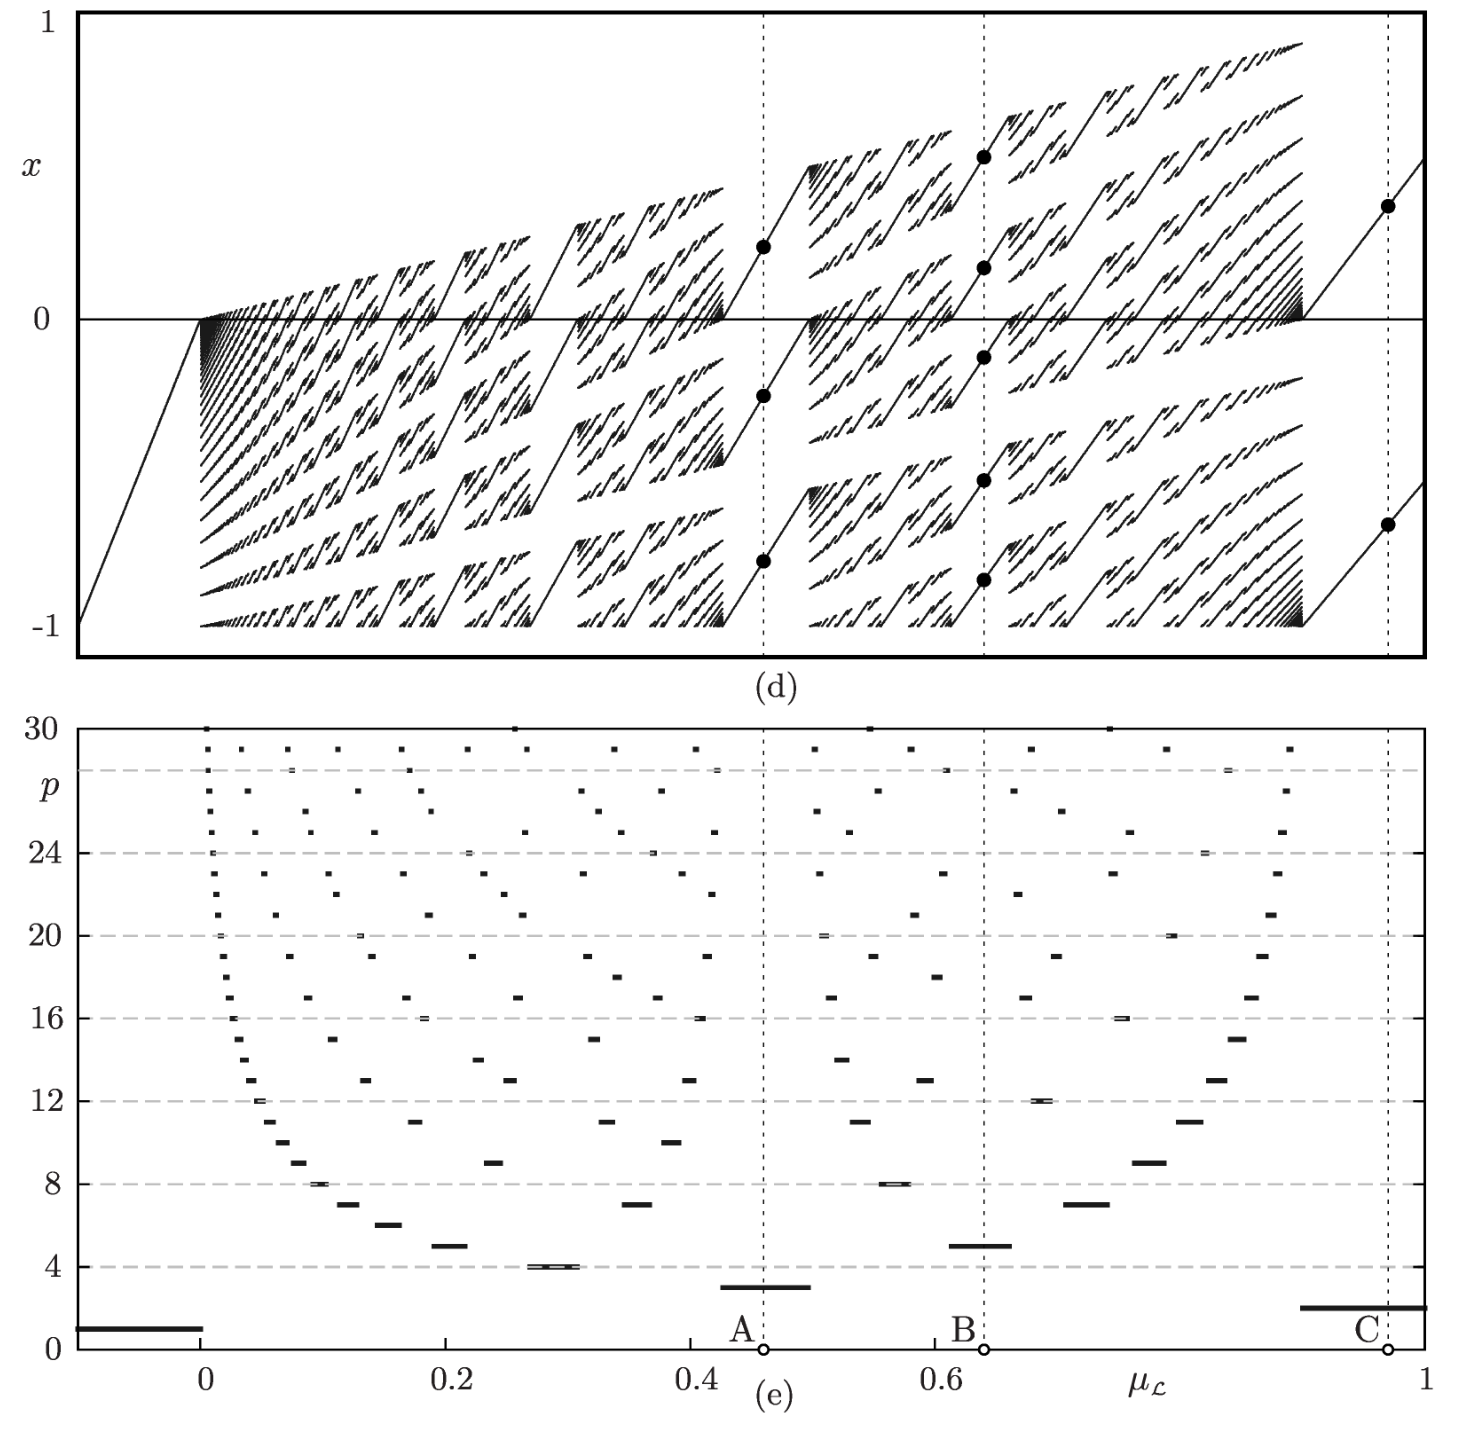
\includegraphics[width=.5 \textwidth]{../StatusMeeting/02/Figs/PeriodAddingDiagrams_Slides.png}
	\caption[Diagram of periods in a period-adding structure between $\L$ and $\R$]{
		Diagram showing the periods of cycles in a period-adding structure with the starting cycles $\L$ and $\R$.
	}
\end{figure}

Next we need to look at a concept called rotation numbers.

\begin{definition}[Rotation Numbers --- Keener]
	Let $\sigma$ be a cycle of a model $x_{n+1} = f(x_n)$ with two branches, $\L$ and $\R$.
	Then the rotation number $\rho(\sigma)$ of this cycle is defined as the fraction of the symbols $\L$ in the symbolic sequence of the cycle $|\sigma|_\L$ divided by the period of the cycle $|\sigma|$.
	\begin{align}
		\rho(\sigma) = \dfrac{|\sigma|_\L}{|\sigma|}
	\end{align}
	\vspace{-4.5em}
	\begin{flushright}
		\cite{Keener80}
	\end{flushright}
\end{definition}

The rotation numbers of the cycles in a period-adding structure are organized in a Farey-tree.
A Farey-tree has two ``root nodes'' and the child node of two nodes is the Farey-sum of the parent nodes~\cite{granados14adding}.

\begin{definition}[Farey-sum]
	The Farey-sum $a \oplus b$ of two fractions $a = \frac{a_1}{a_2}$ and $b = \frac{b_1}{b_2}$ is defined in the following way.
	\begin{align}
		a \oplus b = \frac{a_1}{a_2} \oplus \frac{b_1}{b_2} = \dfrac{a_1 + b_1}{a_2 + b_2}
	\end{align}
\end{definition}

\Cref{fig:state.discont.adding.farey.rot} shows such a Farey-tree of a period-adding structure between two fixed points, $\L$ and $\R$.
If we replace the content of the nodes with the symbolic sequences of the cycles, we get the tree shown in \Cref{fig:state.discont.adding.farey.rot}.
Instead of Farey-addition, here the child node of two parent nodes is the concatenation of the symbolic sequences in the parent nodes.
This explains, why the rotation numbers in the tree in \Cref{fig:state.discont.adding.farey.rot} follows Farey-addition~\cite{granados14adding}.

\begin{theorem}[Rotation Numbers of Concatenated Cycles]
	The rotation number of the concatenation of two cycles $\rho(\sigma\varrho)$ is the Farey-sum of the rotation numbers of both cycles, $\rho(\sigma) \oplus \rho(\varrho)$.
\end{theorem}

\begin{proof}
	\begin{align*}
		\rho(\sigma\varrho)
		= \dfrac{|\sigma\varrho|_\L}{|\sigma\varrho|}
		= \dfrac{|\sigma|_\L + |\varrho|_\L}{|\sigma| + |\varrho|}
		= \dfrac{|\sigma|_\L}{|\sigma|} \oplus \dfrac{|\varrho|_\L}{|\varrho|}
		= \rho(\sigma) \oplus \rho(\varrho)
	\end{align*}
\end{proof}

\begin{figure}
	\centering
	\subfloat[Rotation Numbers]{
		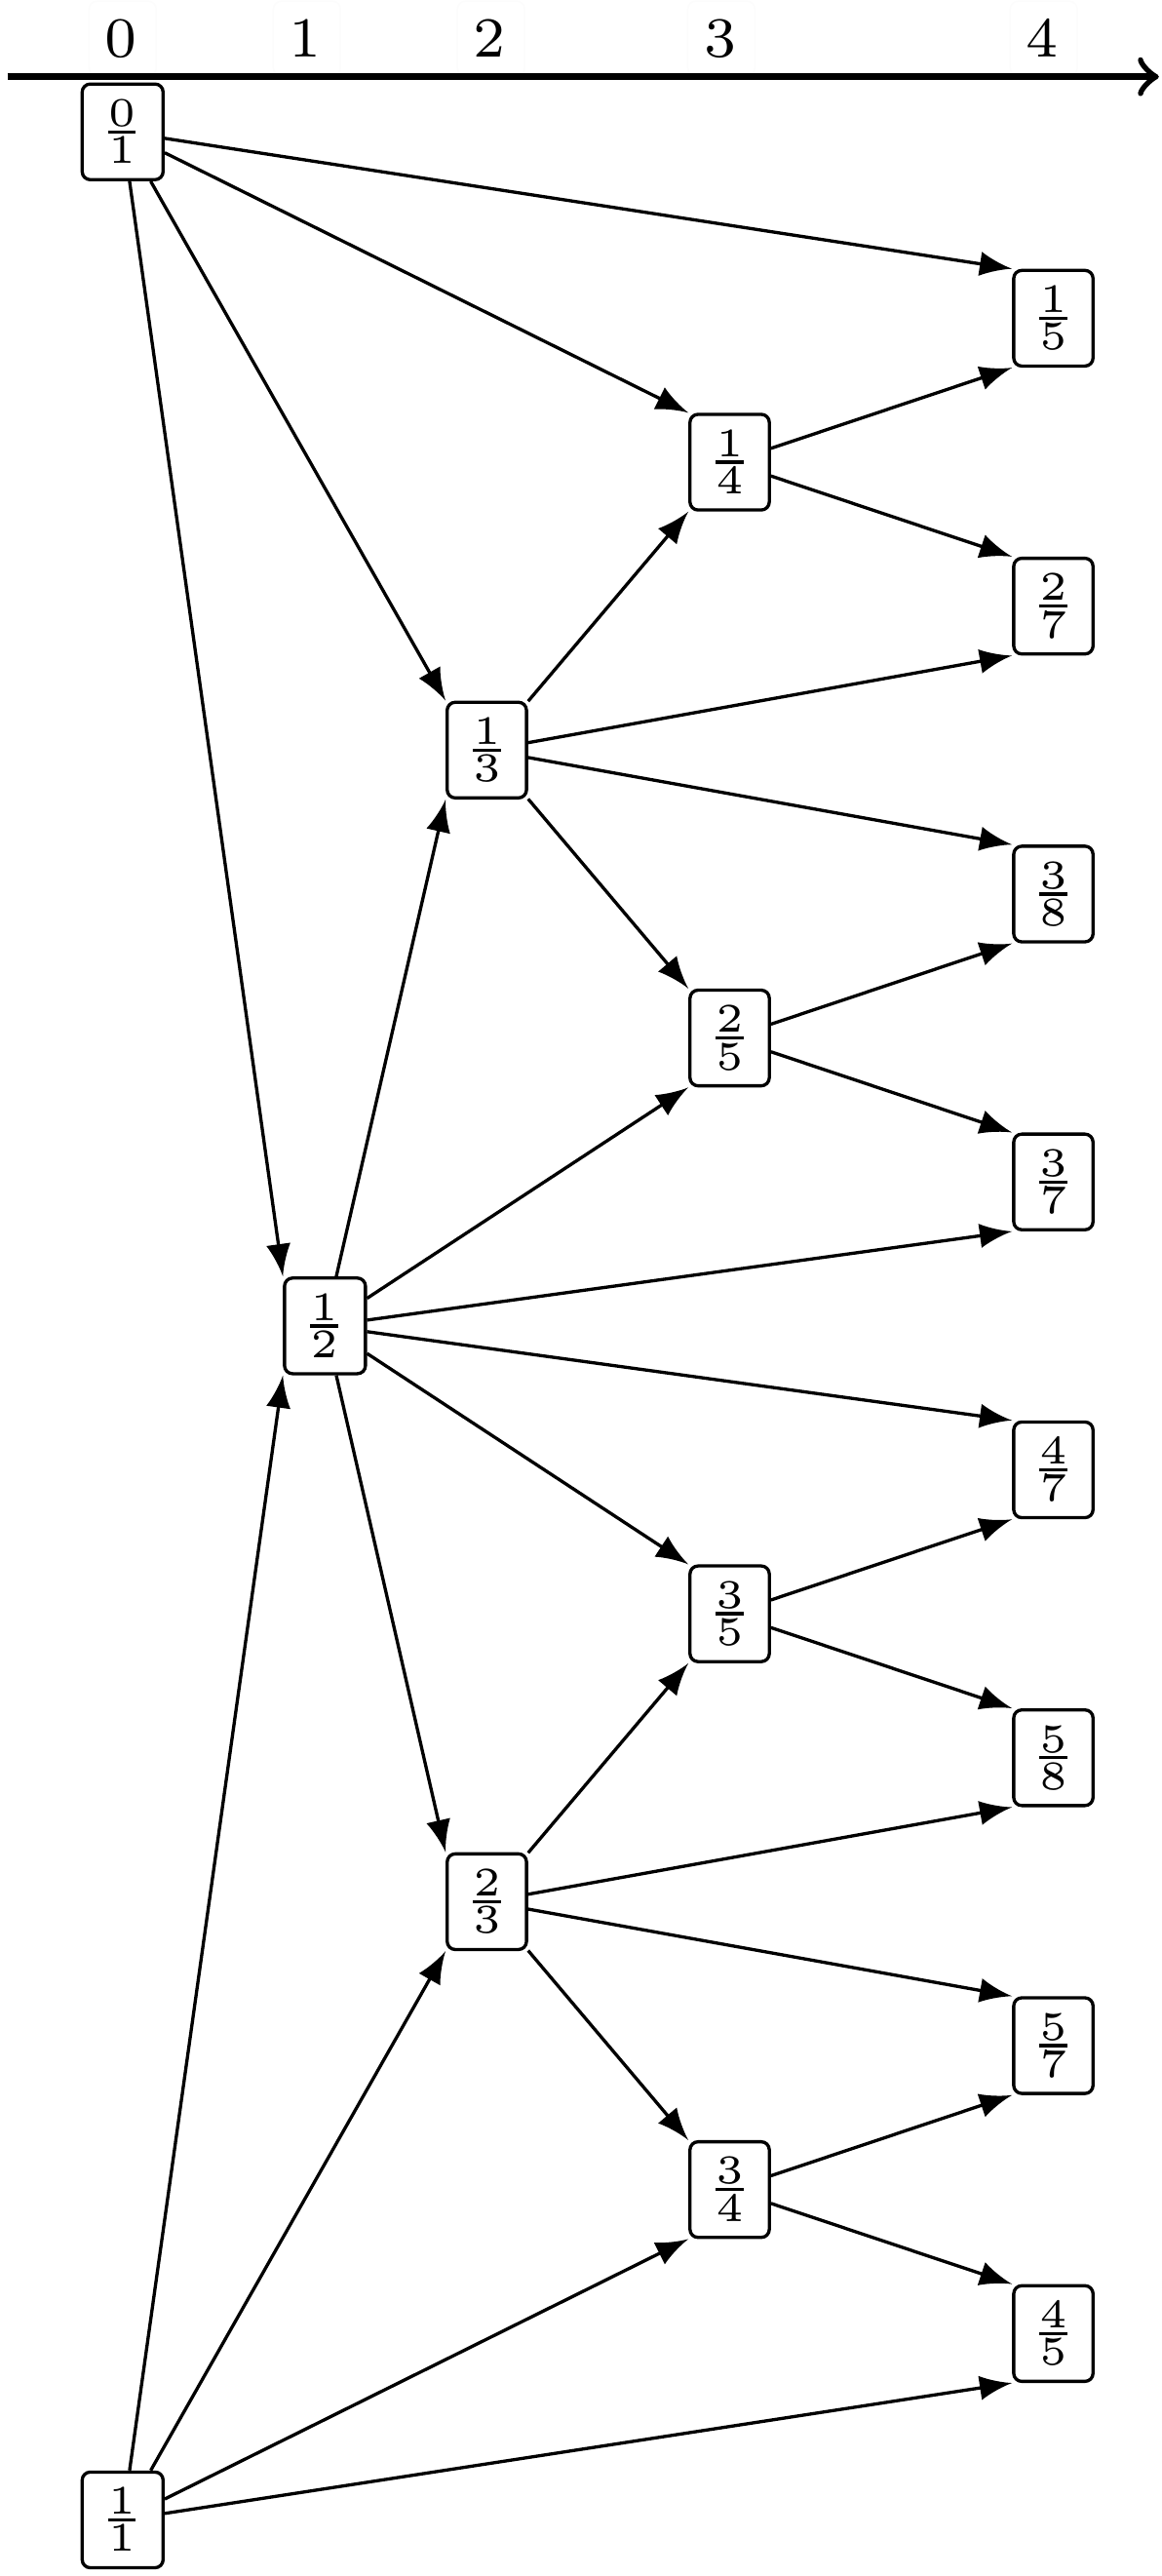
\includegraphics[height=.4 \textheight]{Figures/FareyTrees/LR_RotNum/adding.png}
		\label{fig:state.discont.adding.farey.rot}
	}
	\quad
	\subfloat[Symbolic Sequences]{
		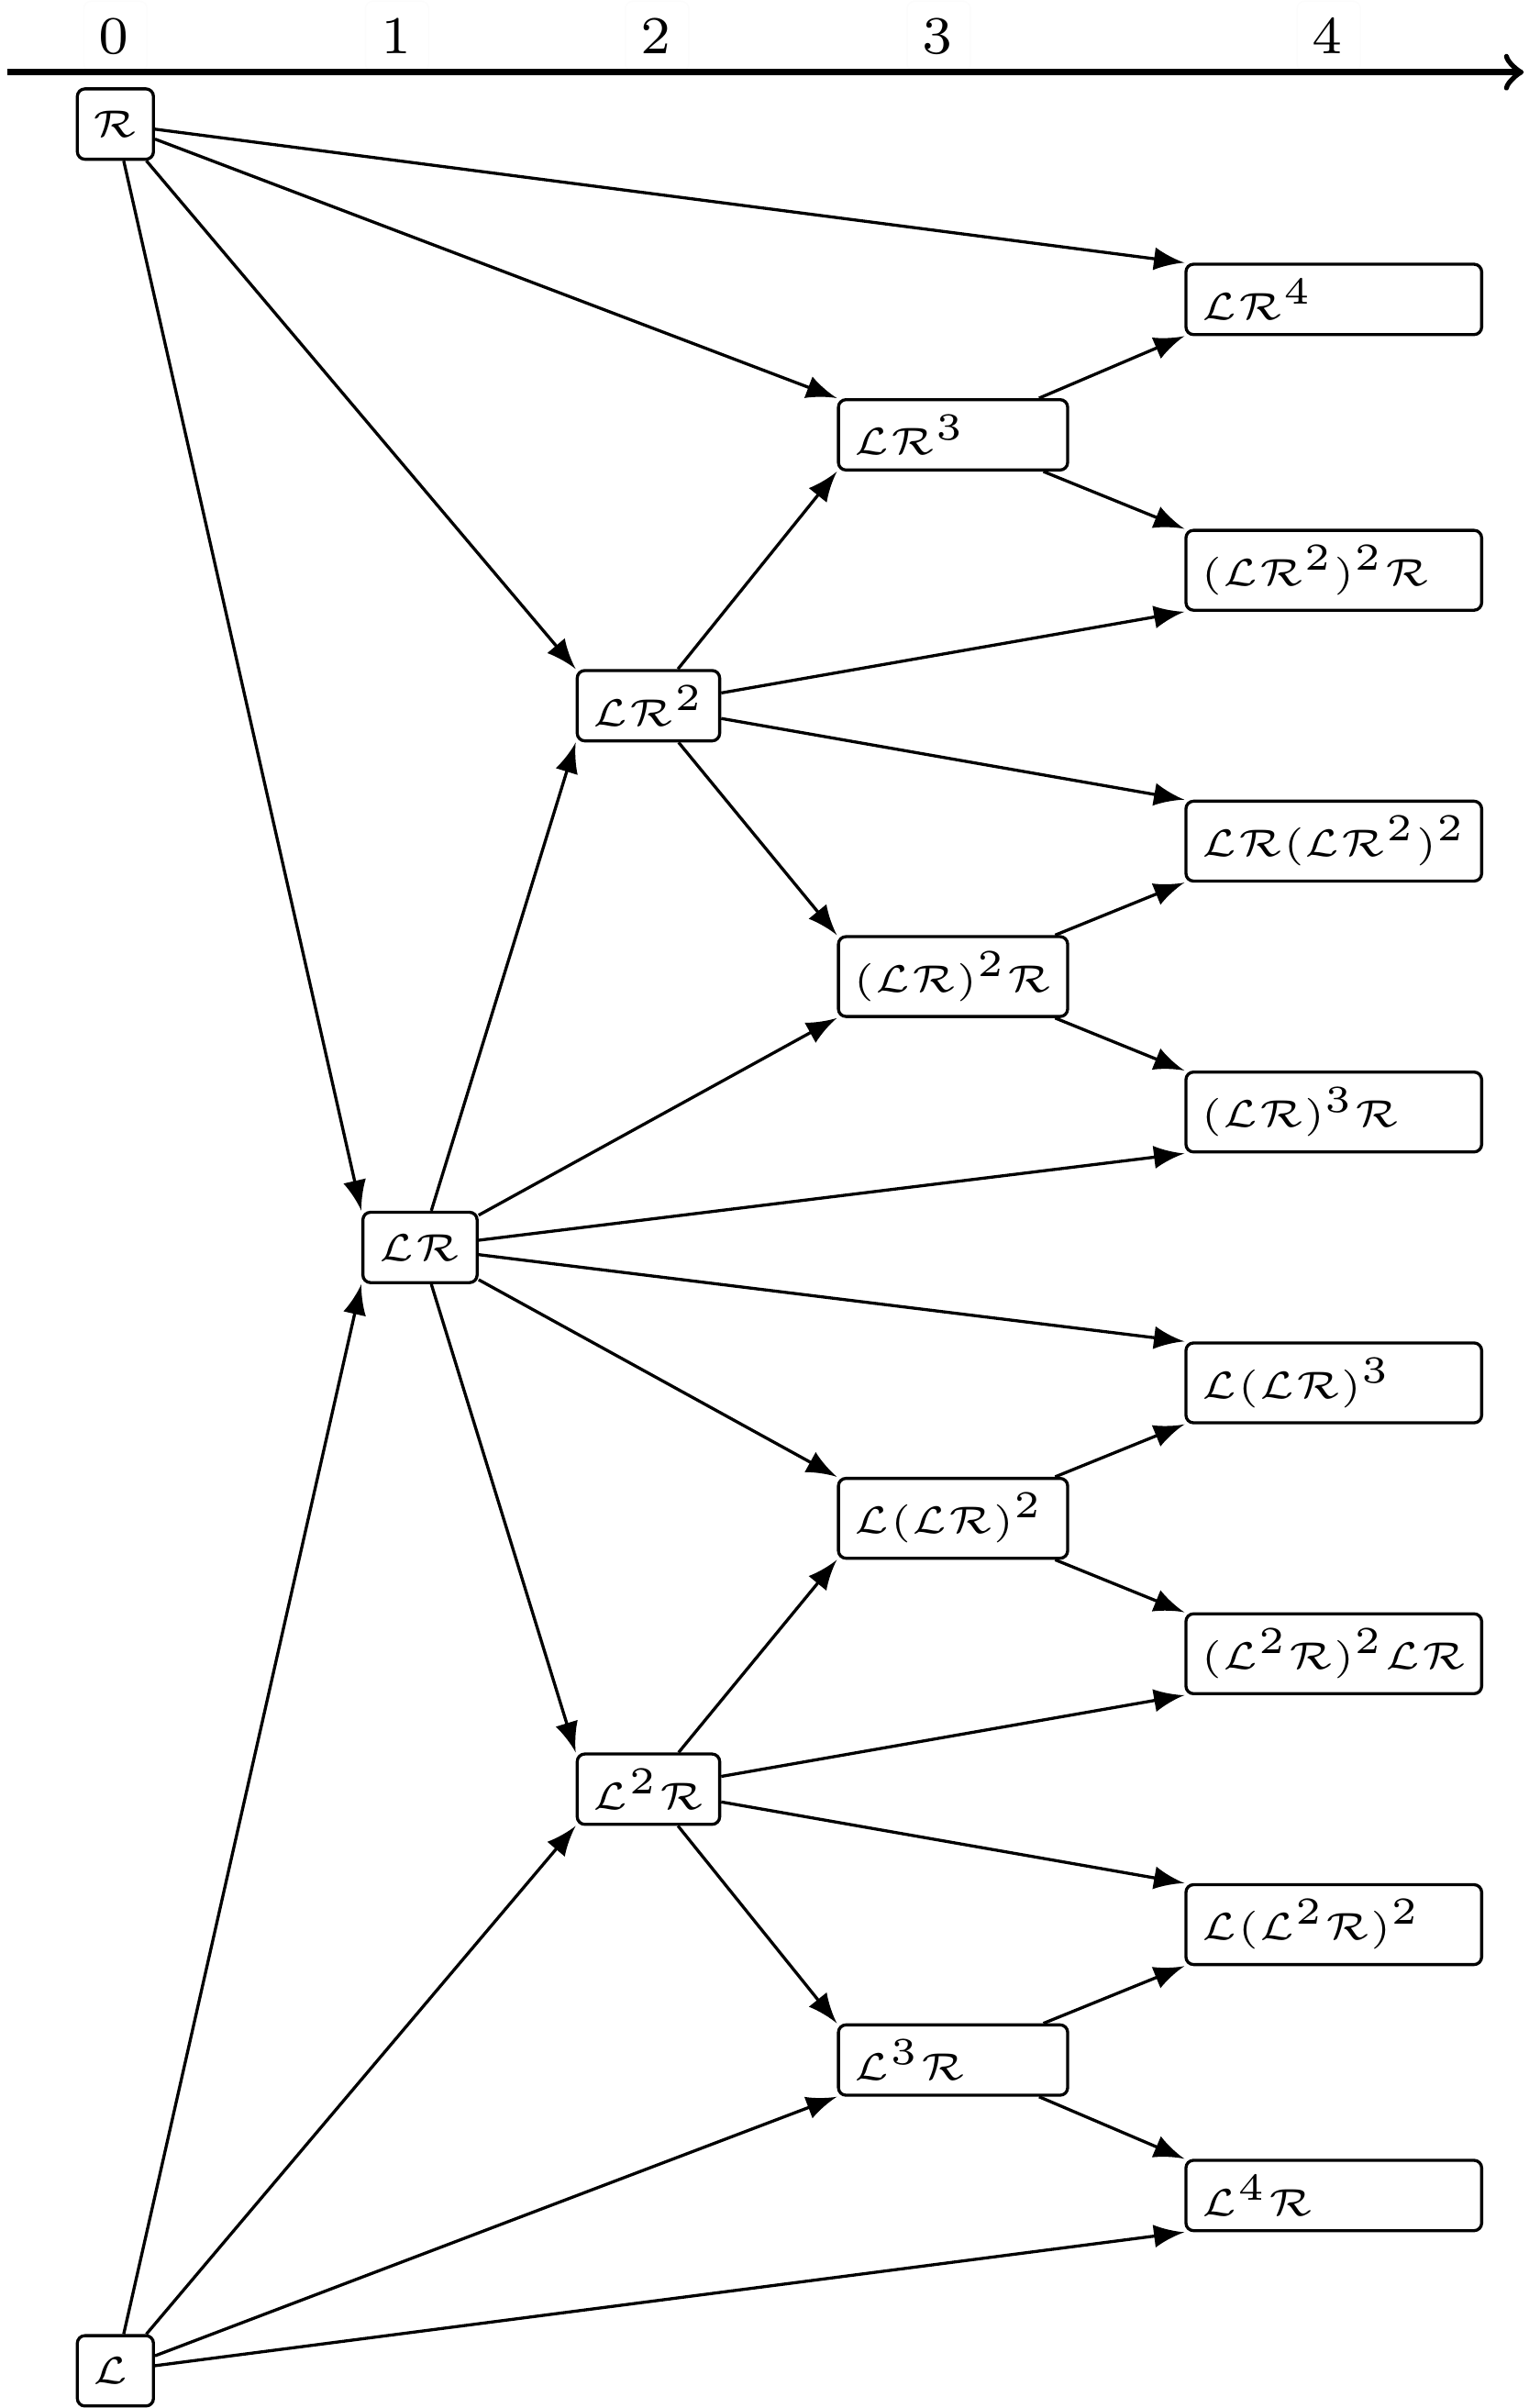
\includegraphics[height=.4 \textheight]{Figures/FareyTrees/LR/adding.png}
		\label{fig:state.discont.adding.farey.sym}
	}
	\caption[Farey-trees of a period-adding structure between $\L$ and $\R$]{
		Farey-trees of a period-adding structure with the starting cycles $\L$ and $\R$.
		(a) Shows the rotation numbers while (b) shows the symbolic sequences of the cycles in this structure.
	}
	\label{fig:state.discont.adding.farey}
\end{figure}
